\begin{figure*}
	\centering
		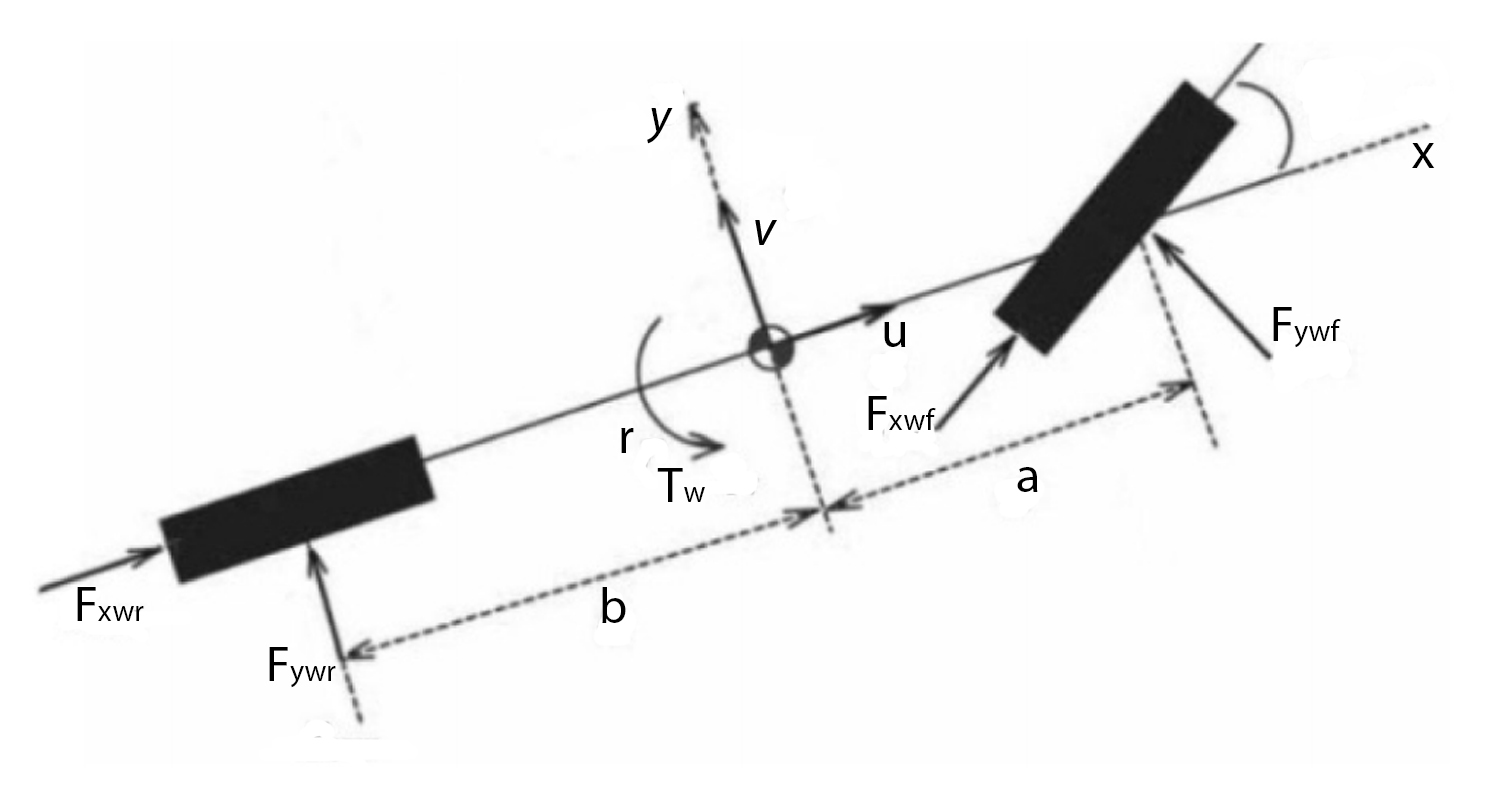
\includegraphics[scale=0.34]{figure/bicyclemodel.jpg}
	\caption{Bicycle model}
    \label{fig:bicyclemodel}
\end{figure*}

\section{Modelling}
In order to determine the tire characteristics with a measurement setup, it is important to use a vehicle model to describe the dynamics of the RC car. Furthermore, the tire characteristics will be described with a model as well. This section describes the vehicle and tire model used in this setup. 

\subsection{The Bicycle Model}
The model used to describe the behavior of the RC Car is the 3 DOF Bicycle Model (Figure \ref{fig:bicyclemodel}) \cite{Liu}. This model consist of the longitudinal (x), lateral (y) and yaw ($\psi$) motion. This model considers that the mass of the vehicle is entirely in the rigid body of the base. Load transfer due to pitch/roll were neglected. This means there is a constant normal force (F\textsubscript{z})  on the wheels. The equations that describe the motion of this model are described as follows:

\begin{subequations}
\begin{align}
    m(\dot{u}-vr) = \sum F_{xi} \quad   (i= f,r) \\
    m(\dot{v}+ur) = \sum F_{yi} \quad   (i= f,r) \\
	I_{z}\dot{r} = F_{yf}a - F_{yr}b\\
	r = \dot{\psi}
    \label{eq:motion}
    \end{align}
\end{subequations}

The longitudinal force (F\textsubscript{xi}) and lateral force (F\textsubscript{yi}) act along the x and y-axis, respectively. The relationship between these forces and the orientation of the wheels are given by equations \ref{eq:bicycle}

\begin{subequations}\label{eq:bicycle}
\begin{align}
	F_{xi} = F_{xwi}\cos\delta_{i}-F_{ywi}\sin\delta_{i} \quad (i=f,r)\\
	F_{yi} = F_{xwi}\sin\delta_{i}+F_{ywi}\sin\delta_{i} \quad (i=f,r)
	\end{align}
\end{subequations}

Where F\textsubscript{xwi} is the longitudinal tire force and F\textsubscript{ywi} is the lateral tire force. 

The difference between the speed of the RC Car and the angular velocity of the wheel is given as a ratio by equation:

\begin{subequations}
\begin{align}
	\kappa =1-\frac{u_{wi}}{R_{w}\omega_{wi}} \quad u_{wi}\leq  R_{w}\omega_{wi} \quad (acceleration)\\
	\kappa = \frac{R_{w}\omega_{wi}}{u_{wi}} -1 \quad u_{wi}> R_{w}\omega_{wi} \quad (Braking)
	\label{eq:kappa}
\end{align}
\end{subequations}

This equation is known as the \textbf{longitudinal slip ratio}, where R\textsubscript{w} stands for the radius of the wheels and $\omega$\textsubscript{wi} for the angular velocity of the wheels. The following equations are used to calculate the  slip angle, where $\alpha\textsubscript{f}$ and $\alpha\textsubscript{r}$ are the \textbf{slip angles} for the front and rear tires, respectively. 
\begin{subequations}
\begin{align}
    \label{eq:alpha1}
	\alpha_{f} = \delta_{f}-\frac{v+ar}{u_{wf}}\\
	\alpha_{r} = \frac{br-v}{u_{wr}}
	\label{eq:alpha2}
\end{align}
\end{subequations}



\subsection{The Magic Formula}	
%eerste zin moet nog iets anders
Since it is necessary to know how the tires would behave in a combined slip condition, not all tire models are suitable. Three models that are able to model this behavior  are: The Dugoff model,The Brush Model and The Magic Formula of Pacejka \cite{Pacejka}. The model used in this experiment is the Magic Formula of Pacejka (Figure \ref{fig:MagicFit}). This semi-empirical model is the most accurate of these three. Another major advantage of this model is that it is described by one single equation. The Dugoff model and the Brush model use separate equations for the linear and non-linear regime, which is a major drawback due to the difficulty in determining at which moment at which region the car is operating \cite{uil}.The general Magic Formula has the following form:

\begin{equation}
	y = D\sin (Ctan^{-1}(Bx-E(Bx-tan^{-1}(Bx)))) \quad
    \label{eq:magicf}
\end{equation}

This equation is valid in the case of pure longitudinal slip or in the case of pure lateral slip. In the case of pure longitudinal slip y is replaced with F\textsubscript{x} and x is replaced with $\kappa$. In the case of pure lateral slip y is replaced with F\textsubscript{y} and x with $\alpha$. The data of y and x are measured and the variables B,C,D, and E are used to fit the formula to the data.

When combined slip occurs the formula changes to:
\begin{subequations}
\begin{align}
\begin{split}
F_{x}&=\cos(C_{x\alpha}\tan^{-1}(B_{x\alpha}tan\alpha))\\
& \quad *D_{x}\sin(C_{x}tan^{-1}tan(B_{x}\kappa-E_{x}(B_{x}\kappa-tan^{-1}(B_{x}\kappa)))\\
\end{split} \label{eqmagiccombined1}\\
\begin{split}
F_{y}&=\cos(C_{y\kappa}tan^{-1}(B_{y\kappa}\kappa))\\
& \quad *D_{y}*sin(C_{y}tan^{-1}(B_{y}\tan\alpha\\
& \quad -E_{y}(B_{y}\tan\alpha-\arctan(B_{y}\tan\alpha))))\\
\end{split} \label{eq:magiccombined2}
\end{align}
\end{subequations}


\begin{figure}[h!]
	\centering
		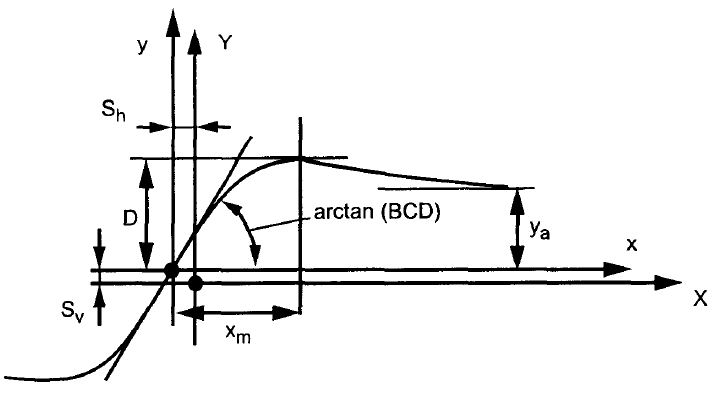
\includegraphics[scale=0.4]{figure/Magic_Formula.png}
	\caption{ Pacejka Magic Formula for tire modeling}
    	\label{fig:MagicFit}
\end{figure}
